\section{ Web-Programmierschnittstelle (Web-API)}
% Einleitung, Motivation
Die Webseite der Wetterstation bietet den interessierten Personen Informationen zum aktuellen Wetter in Arbon. Diese Informationen sind aber nicht nur für Menschen interessant, sondern auch für andere Computer beziehungsweise Server. Das Seebad Arbon zum Beispiel möchte die Wassertemperatur der Wetterstation auf ihrer Webseite anzeigen. Um die Kommunikation von Server zu Server zu vereinfachen werden maschinenlesbare Schnittstellen eingesetzt, sogenannte application programming interfaces (API). Abbildung\,\ref{img:humanvsmachine} zeigt den Unterschied der beiden Darstellungsarten. Auf der linken Seite ist die für den Menschen grafisch mit Farben und Formen aufbereitete Information der Lufttemperatur, auf der rechten Seite die schlichte und rein textbasierte Maschinenversion.

\begin{figure}[htbp!]
  \fbox{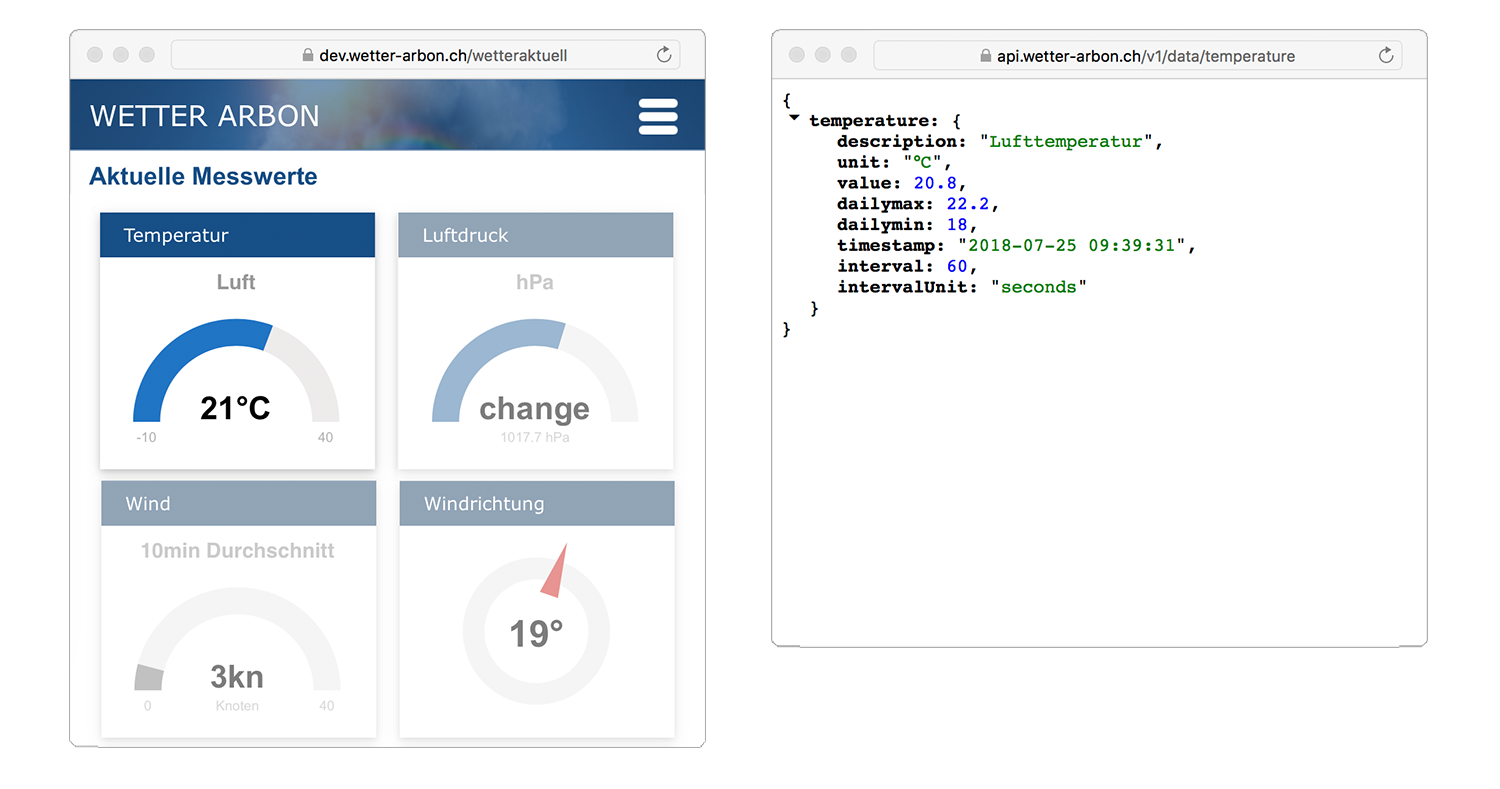
\includegraphics[width=\textwidth-2\fboxsep-2\fboxrule]{img/humanvsmachine}}
	\centering
	\caption{Grafische vs. maschinenlesbare Darstellung}
	\label{img:humanvsmachine}
\end{figure}

%% ############################################################################
%% Unterkapitel
%% ############################################################################
\subsection{Konzipierung und Design der API}
% muss erweiterbar sein
% intuitiv
% einfach
% kurze URL
% DE oder EN?


\subsubsection{Hierarchische Gliederung der Daten}
Die Programmierschnittstelle liefert die aktuellen Messwerte der Wetterstation, Zusatzinformationen, und Infos zur Webcam. Diese Unterteilung wurde bei der Strukturierung der Daten berücksichtigt.

\begin{itemize*}
\item
\item
\item
\end{itemize*}

Wie in Abbildung\,\ref{img:hierarchie} ersichtlich, stellt die Versionsnummer den Ausgangspunkt dar. Danach gibt es die drei Untergruppen misc, webcam und data. Unter data werden alle Informationen, die von der Wetterstation direkt oder indirekt gemessen werden angezeigt. Unter webcam ist der Link zu Webcam aufgeführt und unter misc sind die Zusatzinformation die Sturmwarndaten für die drei Region Bodensee Ost, Mittel und West aufgeführt. Die Struktur wurde so gewählt, dass sie logisch ist, sich beliebig erweitern lässt und die URL trotzdem möglichst kurz ist. Denn die URL entspricht genau dieser hierarchischen Datenstruktur. Um zum Beispiel die aktuellen Lufttemperatur zu erhalten muss folgende URL verwendet werden: \url{https://api.wetter-arbon.ch/v1/data/temperature}. Wenn mehrere Werte auf einmal abgefragt werden sollen, kann die URL eine oder zwei Stufen höher aufgerufen werden also zum Beispiel \url{https://api.wetter-arbon.ch/v1/data/} beziehungsweise \url{https://api.wetter-arbon.ch/v1/}. In diesem Fall werden jeweils alle Daten unterhalb der gewählten Hierarchiestufe ausgegeben.


\begin{figure}[htbp!]
  \fbox{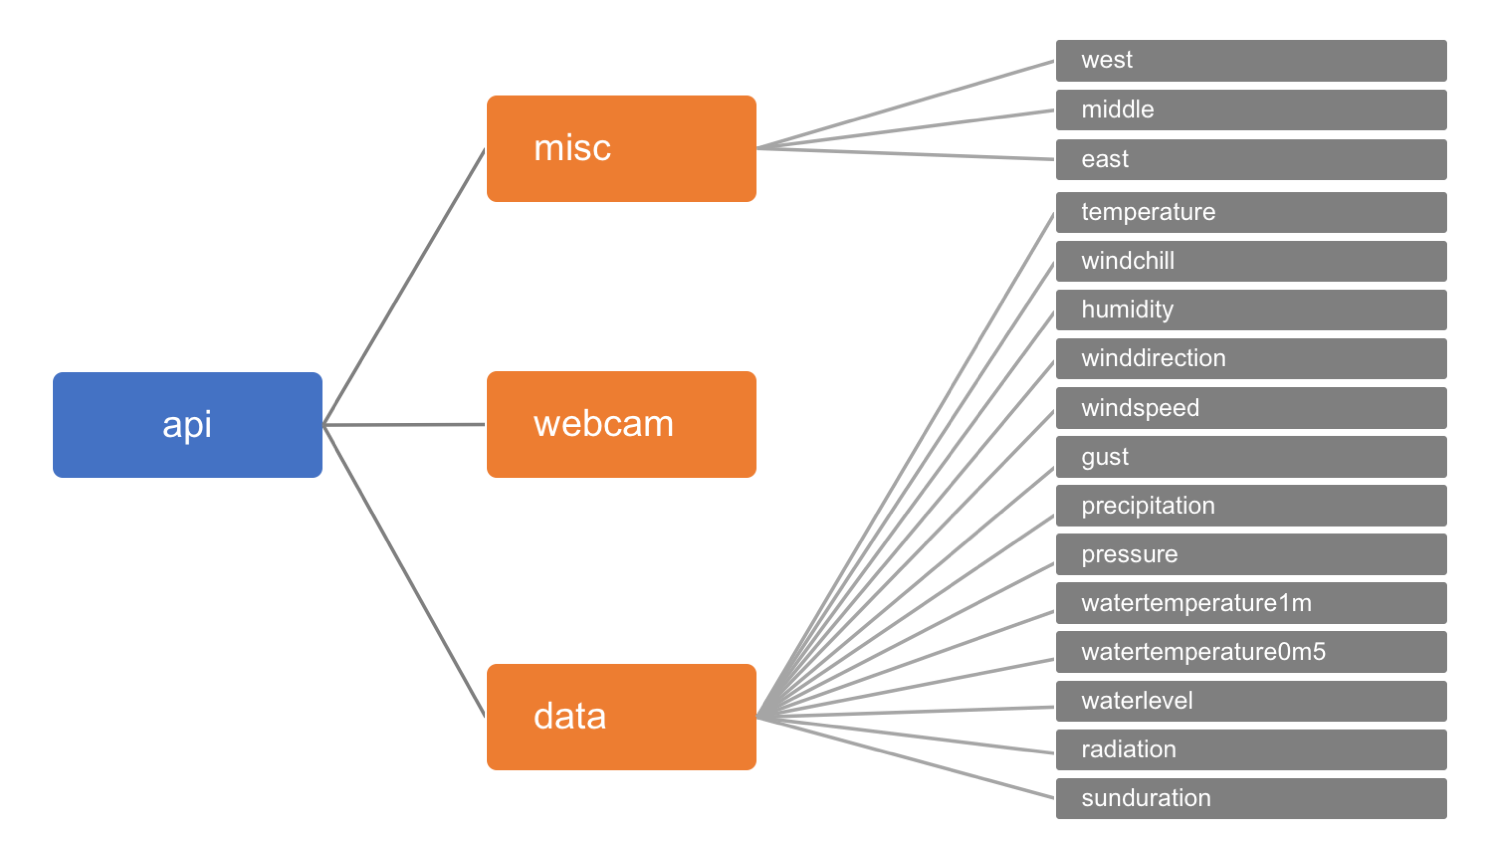
\includegraphics[width=\textwidth-2\fboxsep-2\fboxrule]{img/hierarchie}}
	\centering
	\caption{Dreistufige Datenhierarchie}
	\label{img:hierarchie}
\end{figure}

% Hieraus wird auch die URL entstehen zur Abfrage der Daten. Der Aufruf wird Grundsätzlich über api.wetter-arbon.ch gemacht.
% Um einzelne Werte abzufragen muss tiefer in die Verzeichnisse gegangen werden.




\subsubsection{Anwendung des REST-Prinzips}
Heutzutage werden viele API nach dem REST-Prinzip\,\footnote{REST: Representational State Transfer} von Roy Fielding entwickelt. Der REST-Architekturstil bietet diverse Vorteile unter anderem bezüglich Skalierbarkeit und Sicherheit, wie in der \href{https://www.ics.uci.edu/~fielding/pubs/dissertation/top.htm}{Doktorarbeit}~\cite{Fielding:2000:ASD:932295} von Fielding nachzulesen ist. Eines der wichtigsten Prinzipen daraus ist die Zustandslosigkeit einer Anfrage. Das heisst jede Anfrage vom Client zum Server enthält alle notwendigen Informationen; auf dem Server muss nichts zwischengespeichert werden. REST verwendet zudem die von HTTP zur Verfügung gestellten Methoden\cite{LornaJaneMitchell2013oreilly}. Bei der Wetterstation wird nur die GET-Methode verwendet, da die API der Wetterstation sozusagen ein read-only-Dienst darstellt. Eine Server-Anfrage sieht dann zum Beispiel so aus wie in Listing\,\ref{lst:apirequest}.
\Diskussionspunkt{Was passiert bei POST-Aufruf?}

\vspace{3mm}
\begin{lstlisting}[label=lst:apirequest,caption=Serveranfrage, language=HTML5, style=php]
GET /v1/data HTTP/1.1
Host:           api.wetter-arbon.ch
Cache-Control:  no-cache
\end{lstlisting}
\vspace{3mm}


\subsubsection{Semantische Versionierung}
Versionsnummern unterscheiden einzelne Versionen einer Software, um deren Weiterentwicklungen nachvollziehbar zu kennzeichnen. Die Versionsnummer der API ist beim Aufrufen der oberste Hierarchiestufe sichtbar, siehe Listing\,\ref{lst:versionierung}. Angewendet wird dabei die semantische Versionierung\footnote{\url{https://semver.org}}. Diese teilt die Versionsnummer in folgende drei Bereiche auf: MAJOR.MINOR.PATCH, wobei die drei Bereich unterschiedliche Bedeutungen haben:

\begin{description*}
  \item[MAJOR] Neuerungen hinzugefügt; inkompatibel mit Vorversion
  \item[MINOR] Funktionen hinzugefügt; kompatibel mit Vorversion
  \item[PATCH] Fehler behoben; kompatibel mit Vorversion
\end{description*}

\vspace{3mm}
\begin{lstlisting}[label=lst:versionierung,caption=Versionierungsangabe auf der obersten Hierarchiestufe, language=HTML5, style=php]
{
v1: {
 version: "1.1.1",
 misc:   {...}
 webcam: {...}
 data:   {...}
}
\end{lstlisting}
\vspace{3mm}

\noindent
Die MAJOR-Version unterscheidet demnach zwischen verschiedenen inkompatiblen Versionen. Eine API wird häufig von einem anderen Computer das heisst von einem Programm aufgerufen. Eine inkompatible Änderung würde dazu führen, dass dieses Programm unter Umständen nicht mehr korrekt funktioniert. Aus diesem Grund wurde die MAJOR-Nummer in die URL der API aufgenommen. Auf diese Weise kann parallel eine Version 2 implementiert werden, ohne dass die Nutzer der Version 1 betroffen sind. Die URL setzt sich demnach zusammen aus: \\

\noindent
\texttt{Protokoll://Host/Versionsnummer/Endpunkt}\\
und als Beispiel:\\
\url{https://api.wetter-arbon.ch/v1/data/}

\noindent
\Diskussionspunkt{evt. Erklärgrafik hinzufügen}


\subsubsection{Auswahl des Response-Datenformats}
Damit sich die Computer gegenseitig verstehen, ist es wichtig, dass die Kommunikation in einem standartisierten Datenformat erfolgt. Hier besteht die Möglichkeit zu wählen zwischen JSON, XML oder CSV. Es können auch andere Formate genutzt werden. Wichtig ist jedoch, dass der Server sowie der Client wissen welches Format genutzt wird. Der Server sendet deshalb im Header der Antwort die entsprechende Formatbezeichnung mit (zum Beispiel \texttt{ Content-Type: application/json}). Der Client kann im Header zwar angeben in welchem Format er die Antwort gerne hätte, der Server liefert aber unabhängig davon JSON zurück.

Als Datenformat der API wurde JSON\footnote{JSON: Javascript Object Notation} gewählt, da es sich um ein simples und im Webbereich häufig eingesetztes Datenformat handelt, welches nicht viel Speicherplatz benötigt. Nebst der Lesbarkeit für Maschinen, kann es auch von Menschen einfach gelesen werden. Javascript beispielsweise handhabt JSON nativ und auch die Verwendung in PHP ist simpel, wie im Buch PHP Web Services \cite{LornaJaneMitchell2013oreilly} erwähnt wird. Eine JSON-Antwort mit sämtlichen Werten ist in Anhang Listing \ref{lst:JsonTree} dargestellt. Bei hierarchischen Datenstrukturen spricht man auch von einem Daten-Tree.



%% ############################################################################
%% Unterkapitel
%% ############################################################################
\subsection{Back end Architektur der API}
% Rahmenbedingung: Serverseitige Programmiersprache ist eingeschränkt von Hostpoint auf .......
% Warum wurde php gewählt?
Für die API gibt es jedoch eine wichtige Bedingung. Sie muss in php geschrieben werden, da Hostpoint kein Javascript auf der Serverseite erlaubt.



\subsubsection{Auswahl des PHP-Frameworks anhand einer Nutzwertanalyse}
% kostenlos
% schnell
% einfach und leicht verständlich
% Mittels Nutzwertanalyse ausgewählt
% Sollte es KO-Kriterien geben, werden diese bereits im Vorfeld der Nutzwertanalyse dazu genutzt, die Alternativen für den Vergleich einzuschränken.


% https://www.quora.com/What-is-a-PHP-framework
% https://www.quora.com/Where-can-I-learn-to-create-a-PHP-REST-API-without-using-a-framework
% https://fachinformatiker-anwendungsentwicklung.net/nutzwertanalyse-in-der-projektdokumentation/

% Nutzwertanalyse
\begin{table}[htbp!]
  \setlength\extrarowheight{3pt} % for a more "open" look
  \begin{tabularx}{\textwidth}{|>{\RaggedRight\hspace{0pt}}p{3cm}|p{2.2cm}||p{2.2cm}|X|X|X|}

  \hline
  & \bfseries Gewichtung
  & \bfseries \href{https://codeigniter.com}{CodeIgiter}
  & \bfseries \href{https://www.slimframework.com}{Slim}
  & \bfseries \href{https://lumen.laravel.com}{Lumen}
  & \bfseries ohne\\

  \hline
  \textbf{Dokumentation}
  & xx
  & xx
  & xx
  & xx
  & xx \\

  \hline
  \textbf{Langlebigkeit}
  & xx
  & xx
  & xx
  & xx
  & xx \\

  \hline
  \textbf{Funktions-umfang}
  & xx
  & xx
  & xx
  & xx
  & xx \\

  \hline
  \textbf{Stabilität und Sicherheit}
  & xx
  & xx
  & xx
  & xx
  & xx \\

  \hline
  \textbf{Footprint}
  & xx
  & xx
  & xx
  & xx
  & xx \\

  \hline
  \hline
  \textbf{Total}
  & xx
  & xx
  & xx
  & xx
  & xx \\

  \hline
  \textbf{gewichtet}
  & xx
  & xx
  & xx
  & xx
  & xx \\

  \hline
  \end{tabularx}
  \caption{Nutzwertanalyse der evaluierten php-Frameworks}
  \label{table:php-framework} % label muss NACH caption stehen!!!!
\end{table}


\paragraph*{Kriterien für die Auswahl}
Folgende Kriterien für die Auswahl des php-Frameworks wurden berücksichtigt:
\begin{itemize*}
\item Dokumentation und Einarbeitungszeit: Sind die Funktionen zentral und verständlich dokumentiert?
\item Langlebigkeit: Läuft das Framework auch unter neuen PHP-Versionen?
\item Funktionsumfang: Bietet das Framework Features, die ein produktives Entwickeln ermöglichen (Routing, Header, Response-Formatierung)?
\item Stabilität und Sicherheit: Werden regelmässig Updates zur Verfügung gestellt?
\item Footprint: Ist die Dateigrösse in einem verhältnismässigen Rahmen?
\end{itemize*}




\paragraph*{Gewichtung der Kriterien}
% Gewichtung wird vor der Durchführung des eigentlichen Vergleichs festgelegt
% Gewichtung der Kriterien muss in der Projektdokumentation begründet werden
Die Gewichtungsskala für die Kriterien reicht von 1 (weniger wichtig) bis 4 (sehr wichtig). Für die Auswahl des php-Frameworks wurde folgende Gewichtung vorgenommen:

\begin{itemize*}
\item 4 Kenntnisstand: Da es sich um das Abschlussprojekt des Autors mit fester Zeitvorgabe handelt, ist besonders wichtig, dass die Sprache ihm bereits bekannt ist.
\item 3 Testframeworks: Dem Unternehmen sind automatisierte Tests sehr wichtig und gerade bei Neuentwicklungen sind sie Pflicht.
\item 3 Build-Prozess: Für moderne Konzepte wie Continuous Deployment muss gerade im Webumfeld eine Build-Pipeline vorhanden sein.
\item 2 Funktionsumfang: Gerade im Webumfeld setzt das Unternehmen auf neue Technologien und möchte neue Entwicklungen zeitnah einsetzen.
\item 1 Entwicklungsumgebung: Die IDE kann theoretisch durch einen guten Texteditor abgelöst werden. Daher ist dieses Kriterium nicht ganz so wichtig.
\item 1 Langlebigkeit: Da es sich um eine Webanwendung handelt, die wahrscheinlich häufig an neue Möglichkeiten angepasst werden muss, ist die Langlebigkeit von geringerer Wichtigkeit.
\end{itemize*}




\paragraph*{Bewertungsskala für die Kriterien}
% Skala mit erlaubten Punktwerten und exakte Begründung für die vergebene Punktzahl
% kleine Skala verwenden z.B. 1 bis 3, und definiert exakt, wann welcher Wert vergeben wird.
% unbedingt angegeben, welche Werte gut und welche schlecht sind

Als mögliche Werte für die genannten Kriterien werden die Zahlen 1 (schlecht) bis 3 (gut) verwendet. Im Folgenden wird festgelegt, wann welcher Wert bei den einzelnen Kriterien vergeben wird.

\begin{itemize*}
\item Dokumentation und Einarbeitungszeit
  \begin{enumerate*}
  \item Keine zentrale Dokumentation vorhanden
  \item Zentrale Dokumentation vorhanden, wenig ausführlich
  \item Zentrale Dokumentation vorhanden, ausführlich und verständlich
  \end{enumerate*}
\item Langlebigkeit
  \begin{enumerate*}
  \item Keine Angabe, ob die neue PHP-Version (7.2) unterstützt wird
  \item Neue PHP-Version (7.2) wird unterstützt
  \item Neue PHP-Version werden durch regelmässige Updates unterstützt
  \end{enumerate*}
\item Funktionsumfang
  \begin{enumerate*}
  \item Keine zusätzlichen Funktionen verfügbar
  \item Routineaufgaben sind als Funktionen verfügbar
  \item Routineaufgaben sind als Funktionen verfügbar
  \end{enumerate*}
\item Stabilität und Sicherheit
  \begin{enumerate*}
  \item Wenig verwendet bzw. getestet
  \item Vielverwendet, selten Updates
  \item Vielverwendet mit regelmässigen Updates
  \end{enumerate*}
\item Footprint
  \begin{enumerate*}
  \item Grösser als 5MB
  \item Zwischen 1...5MB
  \item Kleiner als 1MB
  \end{enumerate*}
\end{itemize*}




\paragraph*{Entscheidung für xxxx}
% Nutzwert: stellt das Endergebnis der Nutzwertanalyse dar und repräsentiert die kumulierten bewerteten Kriterien der einzelnen Alternativen.
% Letztlich müssen alle Koeffizienten mit denen der anderen Alternativen verglichen werden, um den Gewinner zu bestimmen
% der einzelne Nutzwert ist nicht aussagekräftig, sondern muss immer ins Verhältnis zu den anderen Ergebnissen gesetzt werden


\subsubsection{MVC-Entwicklungs-Pattern}
- Was ist das MVC-Muster
- Warum wird es bei Web
- Warum ist es bei uns nicht nötig?


Welche Möglichkeiten bietet PHP um dies möglichst einfach umzusetzen? Frameworks? Lösungsansätze
Wie sieht das Funktionsprinzip des gewählten Lösungsansatzes aus?




In diesem Kapitel wird die Funktionsweise nach der Umsetzung des API-Konzepts erklärt. Die ganze API ist Modular aufgebaut, dass diese für weitere Anwendungen oder Messwerte ausgebaut werden kann. Dies beginnt schon beim Verzeichnis (Abb. \ref{img:APIVerzeichnis}) .

% Routing
Für die API ist die Datei path.php essentiell (listing \ref{lst:routing}). Hier wird wie erwähnt das Routing vorgenommen und die entsprechenden Funktionsaufrufe mit den dazugehörenden Parameter.

\vspace{3mm}
\begin{lstlisting}[label=lst:routing,caption=Routing der URL auf die richtige DB-Abfrage, language=php, style=php]
// Beispiel: https://api.wetter-arbon.ch/v1/data/temperature
switch ($url){
 case "/v1/data/temperature":
  createJson(...); break;
 case "/v1/data/windchill":
  createJson(...); break;
 //usw.
\end{lstlisting}
\vspace{3mm}

\begin{figure}[h!]
  \fbox{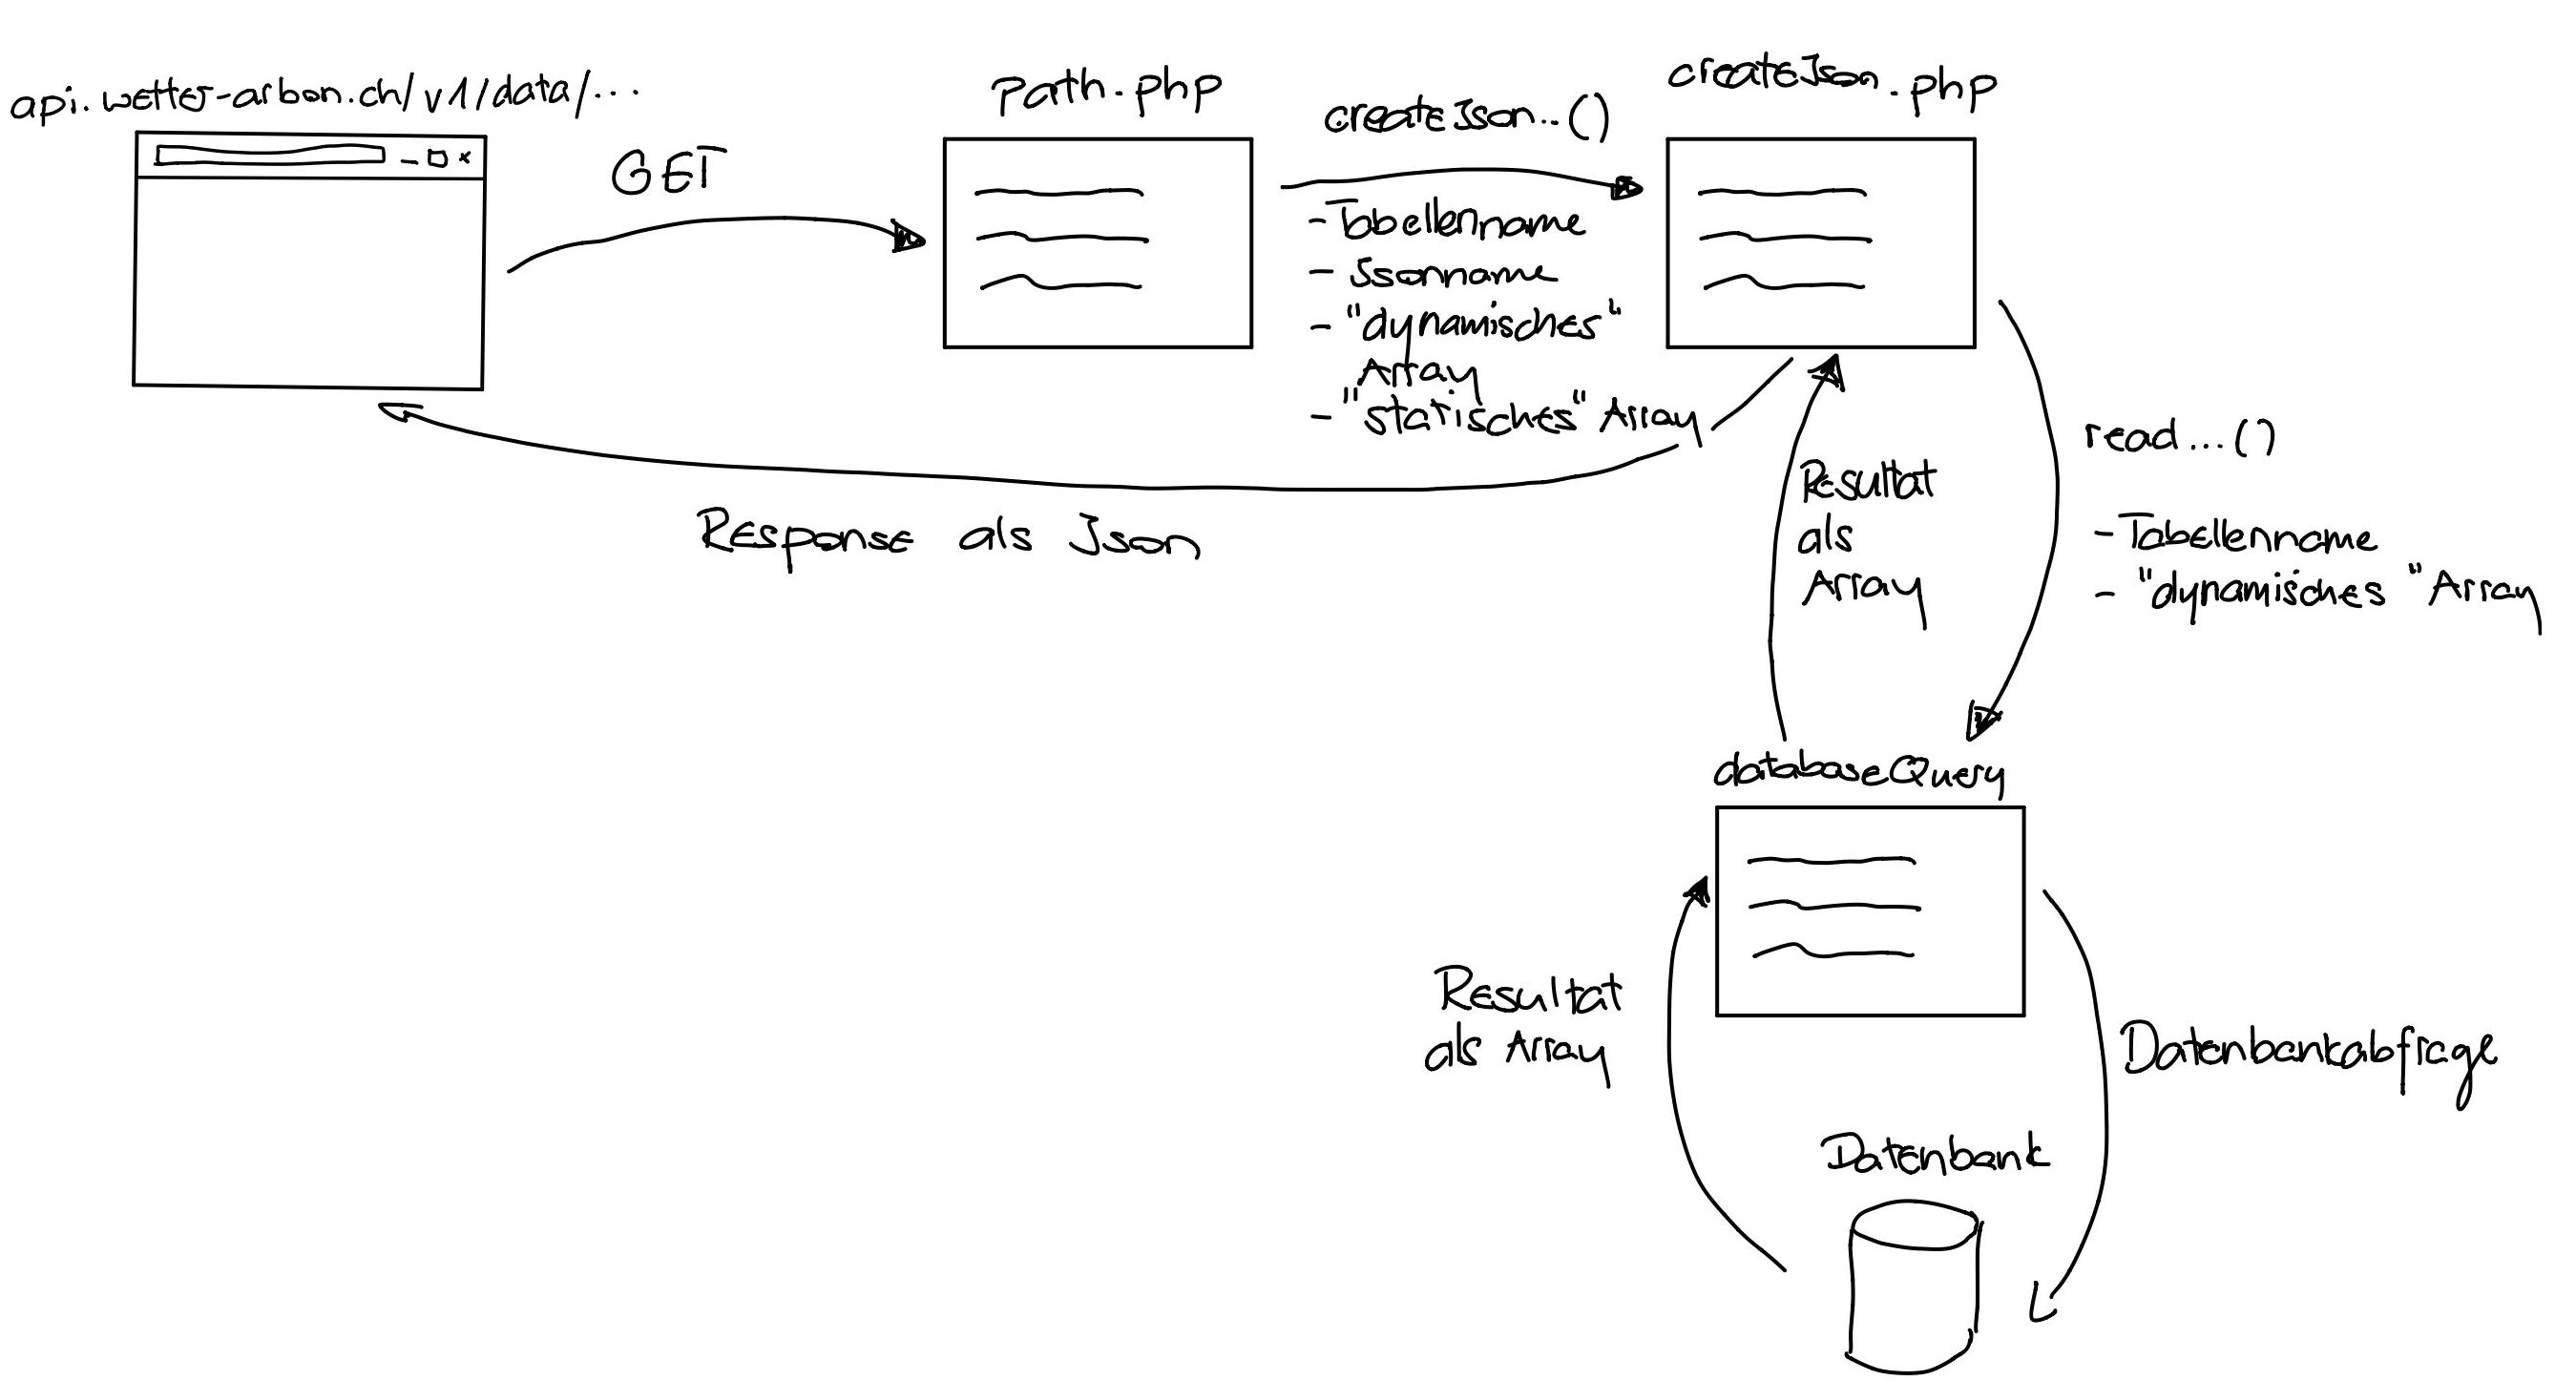
\includegraphics[width=\textwidth-2\fboxsep-2\fboxrule]{img/API_GET.jpg}}
	\centering
	\caption{Ablauf einer API GET-Abfrage}
	\label{img:APIFiles}
\end{figure}



\begin{lstlisting}[label=lst:path,caption=Beispiel Case zuweisung, language=php, style=php]
case "/v1/data/temperature":
	$table = "tblwettertransmitter";
	$requiredData = array(
		"value" => "temperature",
		"min"  	=> "min_daily_temperature",
		"max"   => "max_daily_temperature"
	);
	$dataJsonStatic = array(
	 "description"  => "Lufttemperatur",
	 "unit"  => "C"
	);
	$name = "temperature";
	createJsonMinMax($requiredData, $dataJsonStatic, $table, $name);
	break;
\end{lstlisting}



%% ############################################################################
%% Unterkapitel
%% ############################################################################
\subsection{Online-Dokumentation der API}
postman vs. swagger.io
link zu Doku
%https://documenter.getpostman.com/view/4035921/api-wetter-arbon/RW1XMhBK

Das Verzeichnis V1 beinhaltet drei Unterverzeichnisse, data, misc und webcam. Im Verzeichnis Data wird das JSON der Sensoren aufgebaut, im Verzeichnis Webcam wird das JSON für die Webcam erstellt. Dies ist auch das einzige Verzeichnis welches nicht auf die Datenbank zugreift. Im Verzeichnis misc werden verschiedene Arten von Daten, welche von dritten abgegriffen werden verarbeitet. Nebst dem Verzeichnis, welches modular aufgebaut ist, enthalten auch die Dateien eine gewisse Struktur. Jedes Verzeichnis config enthält die folgenden vier Dateien.


Erfolgt eine GET-Abfrage eines Clients läuft dies gemäss Abb. \ref{img:APIFiles}  ab. Nach der GET-Abfrage wird das Routing anhand des URL Pfades im path.php vorgenommen. Im Case wird der entsprechende Funktionsaufruf mit den Parametern an das CreateJSON übergeben. Hier entsteht zum Schluss auch das JSON. Die Funktion CreateJson...() stellt das JSON nach der Datenbankabfrage read...() in der Datei databaseQuery.php her. Das JSON wird aus dem dynamischen Array, enthält die Messwerte, sowie dem statischen Array, enthält die Einheit und Beschreibung, zusammengesetzt und zurück gegeben.

Die Funktionen sind vom Aufbau her alle gleich. Der Unterschied besteht jedoch beim Aufbau des Json. Für einige Messwerte sind Maximal und Minimalwerte gewünscht. Andere Messwerte hingegen werden in verschiedene Einheiten umgerechnet, damit alle Benutzer die Messwerte auch interpretieren können.
